\documentclass[cn]{homework}

\title{作业6}

\begin{document}
    \maketitle

    \section{平稳性分析}
    通过时序图和ACF\cref{fig:plot acf}可以看出,序列基本上在
    统一水平上下波动,同时自相关系数在一阶之后也很小,
    故判断该序列是平稳的。
    
    \begin{figure}[h]
        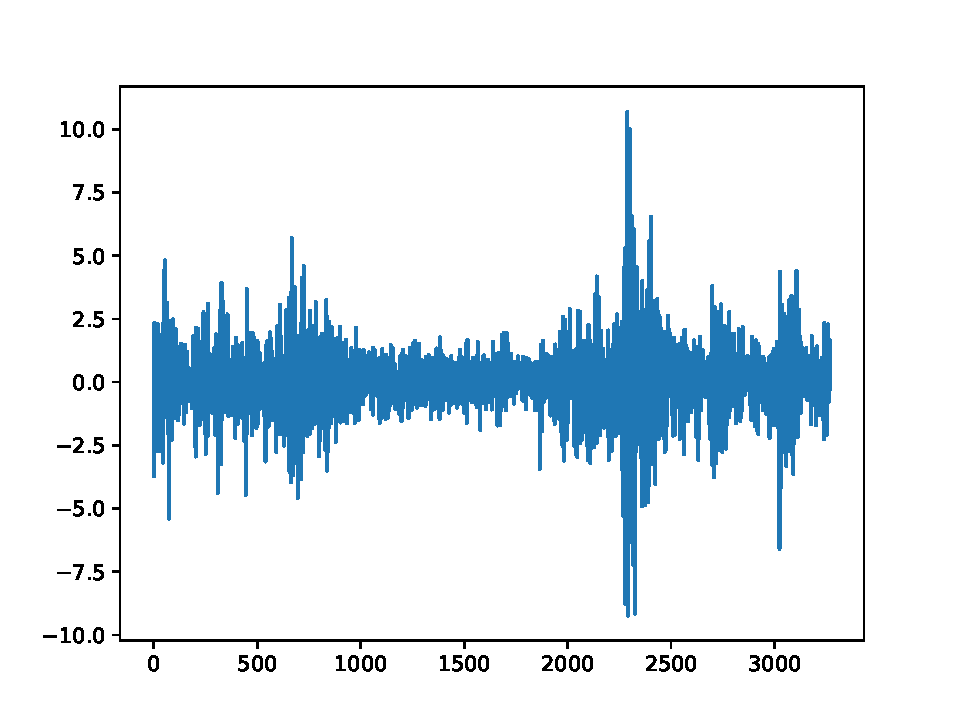
\includegraphics[width=0.47\linewidth]{time-series}
        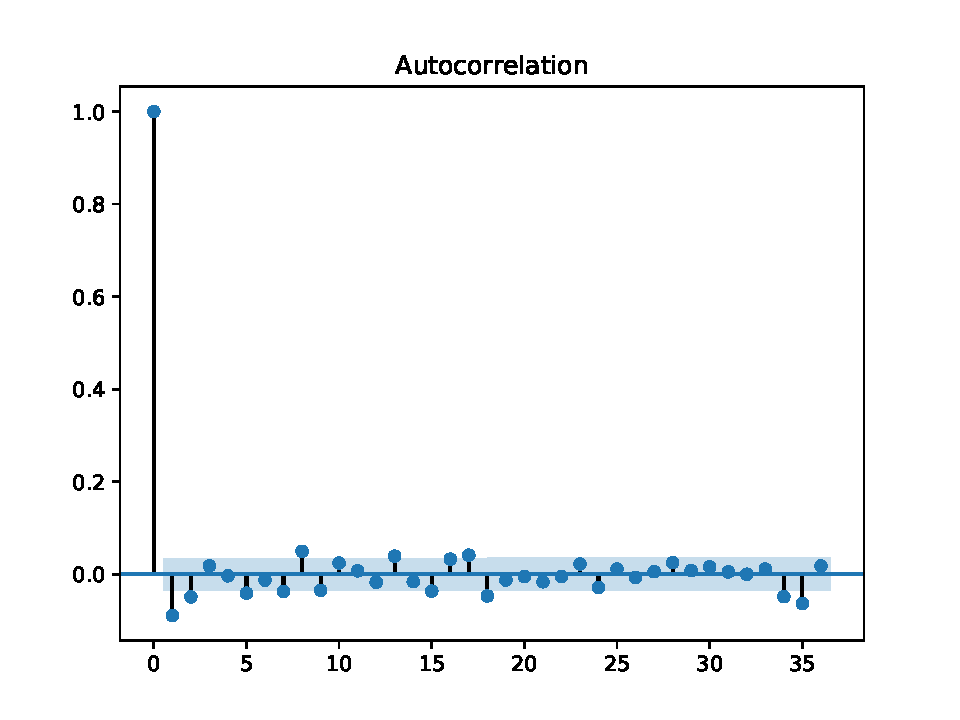
\includegraphics[width=0.47\linewidth]{acf}
        \caption{时序图与ACF}
        \label{fig:plot acf}
    \end{figure}

    \section{ARCH效应检验}
    我们选择合适的AR模型来尝试拟合,经过计算发现,最合适的是AR(2),
    其残差(\cref{fig:resid})表现出了集群效应。

    \begin{marginfigure}
        \centering
        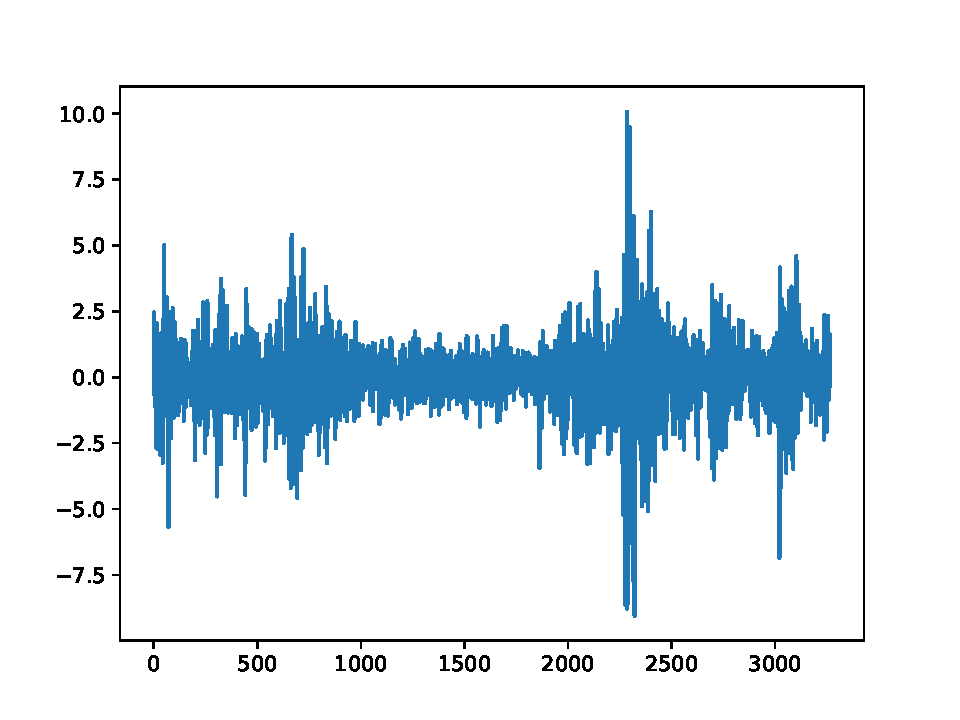
\includegraphics[width=\linewidth]{resid}
        \caption{残差图}
        \label{fig:resid}
    \end{marginfigure}

    而对残差进行LM检验发现(\cref{tab:LM test}),
    许多阶数内ARCH模型均显著成立,具有显著的
    ARCH效应。

    \begin{margintable}
        \centering
        \begin{tabular}{ccc}
            \toprule
            阶数 & LM & $p$\\
            \midrule
            1&    128.122&      0.000  \\
            2&    591.450&      0.000  \\
            3&    613.320&      0.000  \\ 
            4&    652.788&      0.000  \\
            5&    795.432&      0.000  \\
            6&    834.582&      0.000  \\
            7&    884.297&      0.000  \\
            8&    894.295&      0.000  \\
            9&    901.655&      0.000  \\
            10&    906.112&      0.000  \\
            11&    947.015&      0.000  \\
            12&    955.324&      0.000  \\
            \bottomrule
        \end{tabular}
        \caption{LM检验}
        \label{tab:LM test}
    \end{margintable}

    \section{GARCH模型建立}
    考虑使用GARCH(1,1)与GARCH(2,2)来拟合,比较它们的信息准则,
    可以发现虽然GARCH(2,2)更优(\cref{tab:aic}),但是并不明显,以简单起见的原则,
    我们使用GARCH(1,1)。

    \begin{margintable}
        \centering
        \begin{tabular}{ccc}
            \toprule
            模型 & AIC & BIC \\
            \midrule
            GARCH(1, 1) & 9271.99 & 9320.72 \\
            GARCH(2, 2) & 9295.35 & 9331.90 \\
            \bottomrule
        \end{tabular}
        \caption{AIC \& BIC}
        \label{tab:aic}
    \end{margintable}

    于是可以得到
    \[\left\{\begin{aligned}
        X_t&=0.0437-0.0578X{t-1}-0.0383X_{t-2}+\varepsilon_t\\
        \varepsilon_t&=\sqrt{h_t}e_t\\
        h_t&=0.0138+0.0840\varepsilon_{t-1}+0.9063h_{t-1}
    \end{aligned}\right.\]
    其中$e_t\stackrel{\text{i.i.d.}}{\sim}\mathcal N(0,1)$

    \section{样本内预测}
    对序列进行2012:06:20到2012:07:02的时段进行条件方差预测。
    如\cref{tab:forecast}。
    \begin{table}
        \centering
        \begin{tabular}{ccc}
            \toprule
            ENTRY & 方差预测 \\
            \midrule
            2012:06:20 & 0.9216 \\
            2012:06:21 & 1.2276 \\
            2012:06:22 & 1.1441 \\
            2012:06:25 & 1.2419 \\
            2012:06:26 & 1.1486 \\
            2012:06:27 & 1.1274 \\
            2012:06:28 & 1.0359 \\
            2012:06:29 & 1.3852 \\
            2012:07:02 & 1.2745 \\
            \bottomrule
        \end{tabular}
        \caption{样本内预测}
        \label{tab:forecast}
    \end{table}

    \begin{figure}[h]
        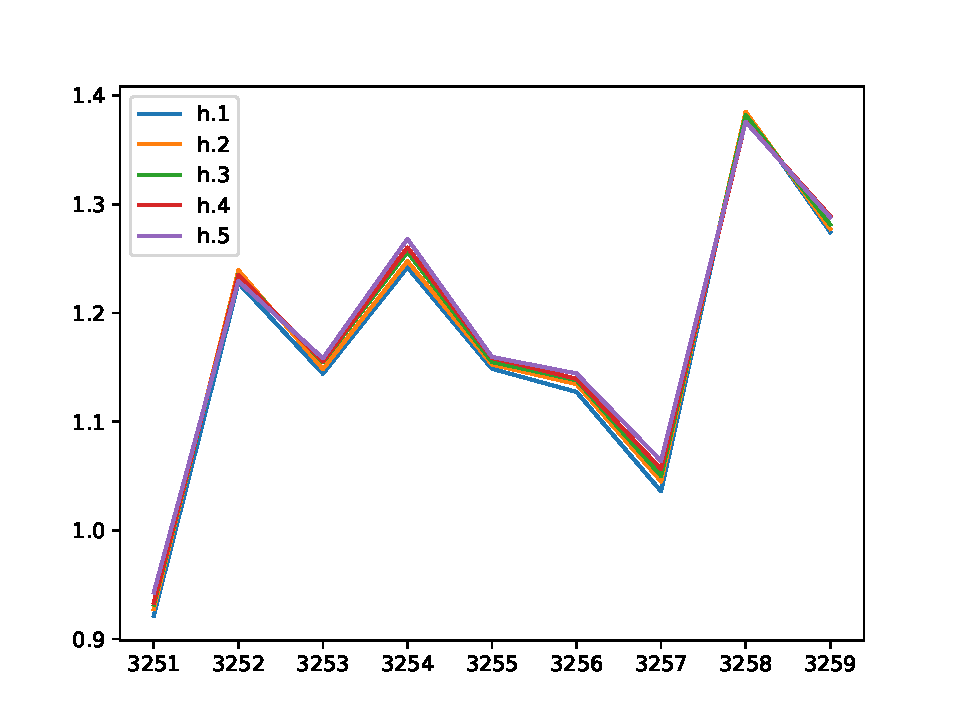
\includegraphics[width=\linewidth]{forecast}
        \caption{方差预测}
        \label{fig:forecast}
    \end{figure}

    \newpage
    \appendix
    \section{Python代码}
    \lstinputlisting[language=Python]{rate.py}
\end{document}